\documentclass{beamer}
\usepackage[utf8]{inputenc}

%Information to be included in the title page:
\title{Seminar Talk \\ F09: Neuromorphic Computing}
\author{Students: Robin Dorstijn \& Moritz Epping \\ Supervisor: Jakob Kaiser}
\institute{Universität Heidelberg}
\date{January 2021}

\begin{document}

\frame{\titlepage}

\begin{frame}
    %%%
    \frametitle{Summary}
    \begin{enumerate}
        \item Theoretical Overview
        \item Results
        \item Discussion
    \end{enumerate}
    %%%
\end{frame}

\begin{frame}
    %%%
    \frametitle{Motivation}
   	\begin{itemize}
   		\item Goals of Neuromorphic Computing:
   		\begin{enumerate}
   			\item Building more efficient computers (Von-Neumann Bottleneck vs.  Evolution)
   			\item  Understanding brain by trying to rebuild it!	
   		\end{enumerate}
   		\bigskip
   		\item Proposed Architecture: SPIKEY (Heidelberg)
   		\begin{enumerate}
   			\item What are basic properties neuromorphic computing devices must fulfill?
   			\item Does SPIKEY fulfill these properties?
   			\item How well can we use it for more complicated purposes?
   		\end{enumerate}
   	\end{itemize}
\end{frame}

\begin{frame}
    %%%
    \frametitle{Theoretical Overview - Neurons}
    \begin{columns}
          \column{0.28\linewidth}
             \centering
             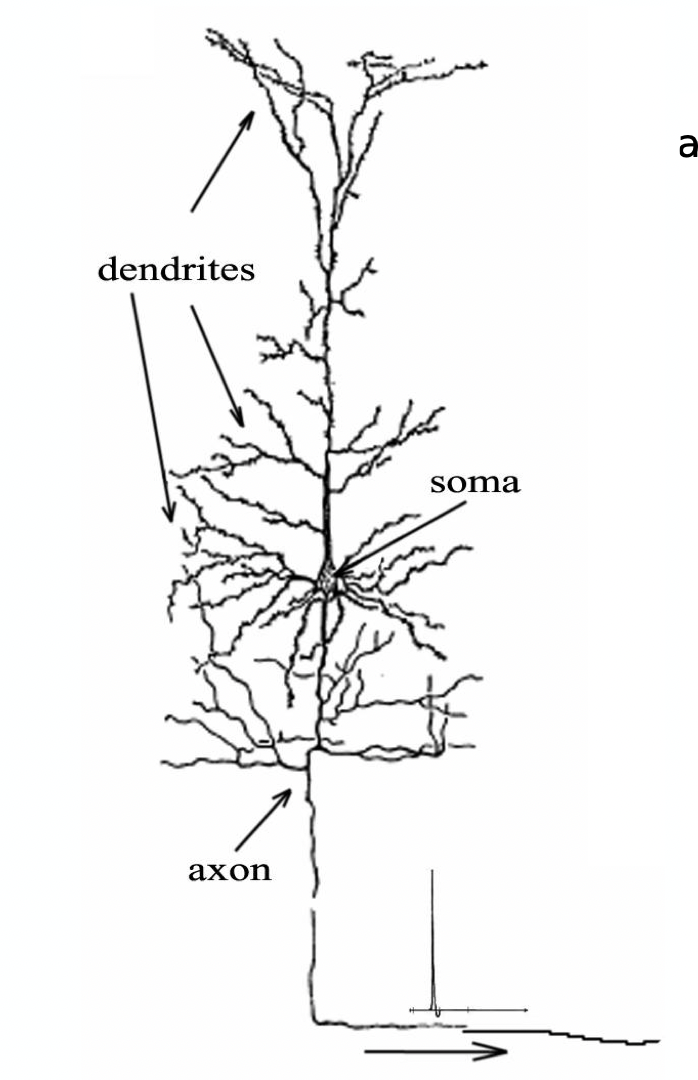
\includegraphics[height=5cm, width=3.5cm]{figures/neuron_script.png}
           \column{0.68\linewidth}
              \begin{itemize}
   	
   				\item Biological Neuron
   				\begin{itemize}
   					\item Basic computational units of the brain
   					\item Electronic information processing
   					\item Receive input signals (ion waves) via \textbf{dendrites}
   					\item Depending on input: Create a signal
   					\item Transmit signal to other neurons
   				\end{itemize}
   				
   				\item form a network with several interconnected neurons
 			\end{itemize}
	\end{columns} 
   	
\end{frame}

\begin{frame}
    %%%
    
    \frametitle{Theoretical Overview - LiF Model}
    
     \begin{figure}
    		\centering
    		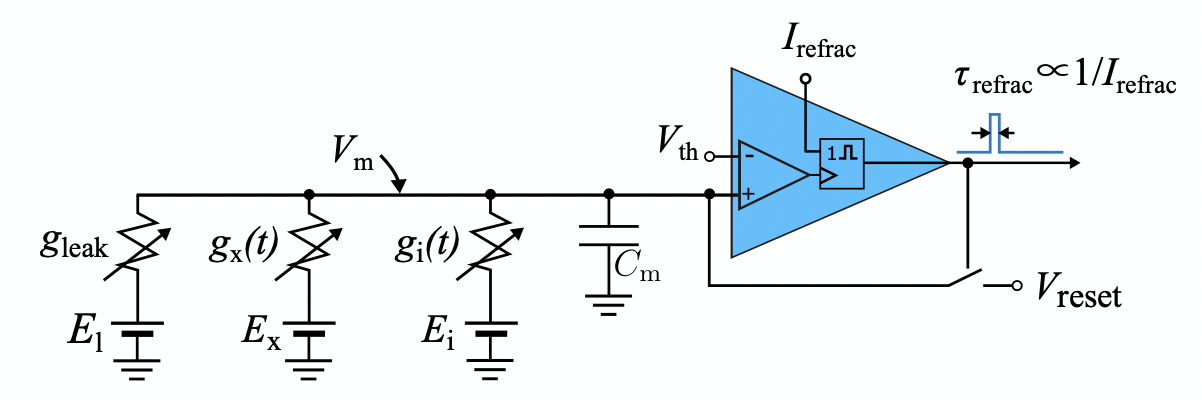
\includegraphics[width=0.8\textwidth]{figures/lif_script.png}
    		%\caption{source: FP09 neuromorphic computing script,  2020}
    \end{figure}
    
     \begin{itemize}
   	
   		\item Electronical Analogy: LIF - Circuit
   		\begin{itemize}
   				\item \textbf{L}eaky \textbf{I}ntegrate and \textbf{F}ire
   				\item Treat neuron as capacitor
   				\item Currents charging / decharging it (input)
   				\item Op-Amp: Compare capacitor voltage to \textit{threshold voltage},  if 
   				$V\geq V_{th}$ then spike
   		\end{itemize}
 	\end{itemize}

\end{frame}

\begin{frame}
	\frametitle{Hardware realization: Spikey}
	\begin{columns}
          \column{0.5\linewidth}
          	\begin{figure}
    				\centering
    				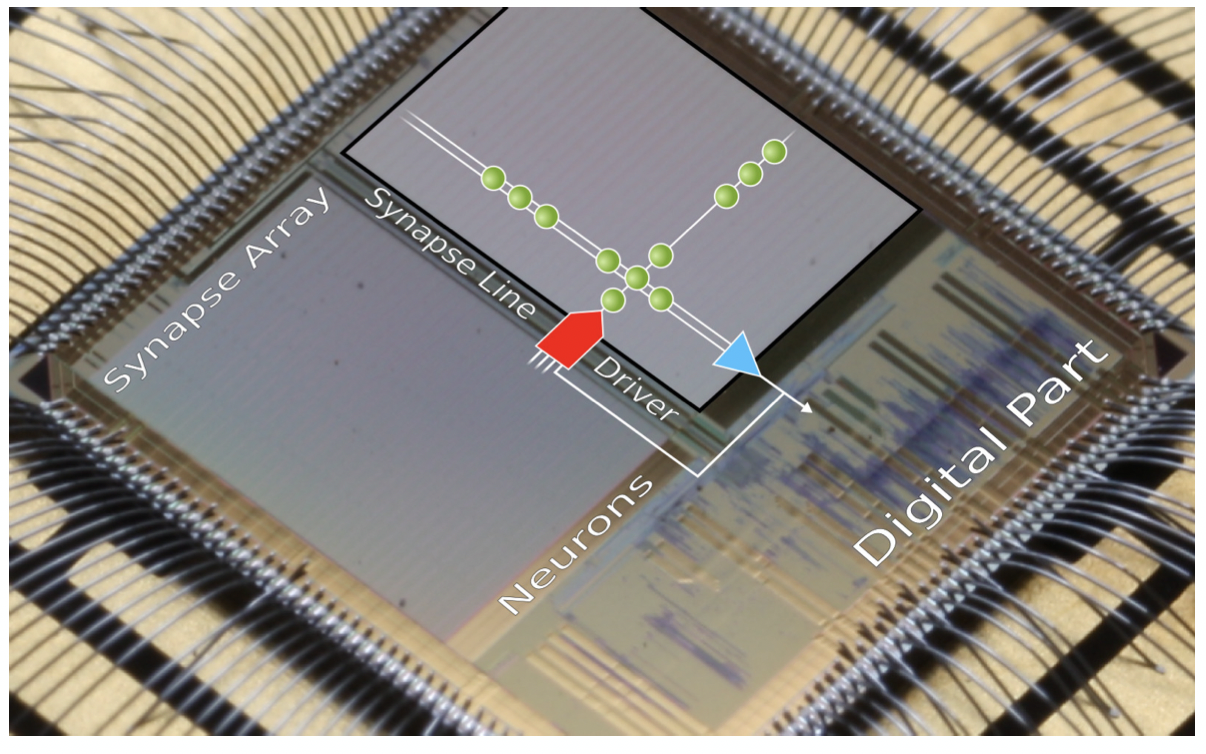
\includegraphics[width=\linewidth]{figures/script_spikey_image.png}
    				%\caption{source: FP09 neuromorphic computing script,  2020}
 		   \end{figure}
 		   \begin{itemize}
          		\item Spikey as a collection of LiF circuits interconnected with synapses
          	\end{itemize}
          
          \column{0.5\linewidth}
          \begin{figure}
    				\centering
    				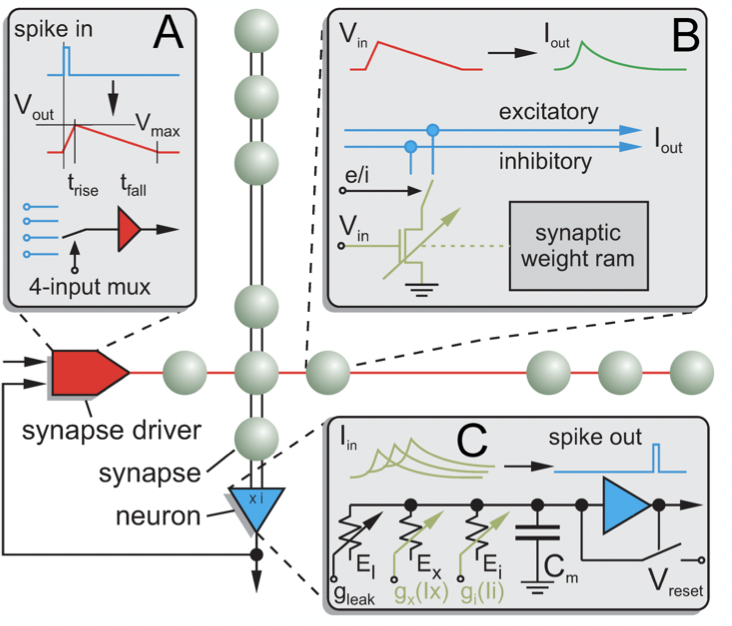
\includegraphics[width=\linewidth]{figures/script_spikey_schematic.png}
    				%\caption{source: FP09 neuromorphic computing script,  2020}
 		   \end{figure}
 		   \begin{itemize}
          		\item Schematic of the basic operation process
          	\end{itemize}
          	
	\end{columns}
\end{frame}


\begin{frame}
    %%%
    \frametitle{Results - basic firing behaviour} 
    %%%    
\end{frame}

\begin{frame}
    %%%    
    \frametitle{Discussion}
    %%%    
\end{frame}

\end{document}
